% ----------- 1. DECLARACIÓN DE CLASE Y OPCIONES -----------
\documentclass[acmsmall, screen=true, review=false]{acmart}

% 'acmsmall': Define el formato de columna simple para journals.
% 'screen=true': Habilita enlaces de colores para visualización en pantalla.
% 'review=false': Deshabilita el modo de revisión (numeración de líneas).

% ----------- 2. PAQUETES (El sistema ACM los carga automáticamente) -----------
\usepackage{tikz} %para graficas
\usetikzlibrary{arrows.meta, positioning, calc, decorations.pathreplacing}
\usepackage{cancel}

% Si usas BibTeX, asegúrate de que use el estilo de citas de ACM (por defecto).
\citestyle{acmnumeric} % Opcional, pero define el estilo de citas (numérico).

% ----------- 3. METADATOS (TOP MATTER) -----------
\acmJournal{TOS} % Reemplaza con la abreviatura real de tu revista ACM
\acmVolume{1}
\acmNumber{1}
\acmArticle{1} %que onda con esto?
\acmYear{2025}
\acmMonth{11} % 11 para noviembre
\setcopyright{acmlicensed}

\title[Teoremas de Jerarquía]{Teoremas de Jerarquía}
\subtitle{Seccion 9.1 Indroducción a la Teoría de la Computación, Michael Sipser}

% Autor 1
\author{Ana Sofía Hernández Zavala}
%\orcid{319316717}
\affiliation{
  \institution{Universidad Nacional Autónoma de México, Facultad de Ciencias}
  \city{Ciudad de México} 
  \country{México} % OBLIGATORIO
}
\email{anasofiahdzz@ciencias.unam.mx}

% Autor 2
\author{Sanluis Castillo Daniela Alejandra}
\affiliation{
  \institution{Universidad Nacional Autónoma de México, Facultad de Ciencias}
  \city{Ciudad de México}
  \country{México}
}
\email{danielasanluisc@ciencias.unam.mx}

% Autor 3
\author{Metzitlalli Álvarez Ríos}
\affiliation{
  \institution{Universidad Nacional Autónoma de México, Facultad de Ciencias}
  \city{Ciudad de México}
  \country{México}
}
\email{metzi.ar18@ciencias.unam.mx}

%checar esto
% Conceptos de Clasificación de Computación ACM (CCS)
% Obligatorio para artículos > 2 páginas.
\begin{CCSXML}
<ccs2012>
 <concept>
  <concept_id>10003033.10003083.10003095</concept_id>
  <concept_desc>Networks~Network reliability</concept_desc>
  <concept_significance>500</concept_significance>
 </concept>
</ccs2012>
\end{CCSXML}

\ccsdesc[500]{Networks~Network reliability}

% Palabras clave (Keywords)
\keywords{teoremas, jerarquías, tiempo, espacio, corolario, definicion, máquina de Turing}

% ----------- 4. COMIENZO DEL DOCUMENTO -----------
\begin{document}

% 1. EL RESUMEN VA PRIMERO, DENTRO DE begin{document}
\begin{abstract}
Este es el resumen de la investigación. (Ya puedes borrar el comentario confuso que estaba aquí).
\end{abstract}

% 2. LUEGO SE GENERA EL BLOQUE DE TÍTULO Y METADATOS
\maketitle

% 3. LUEGO VIENE LA PRIMERA SECCIÓN
\section{Introducción}
El sentido común nos dice que si le damos más tiempo o más espacio a una máquina de Turing entonces debería de incrementar la clase de problemas que podría resolver; y los Teoremas de Jerarquía lo confirman, ya que estos teoremas prueban que las clases de complejidad de tiempo y espacio no son todas las mismas. \\
Por ejemplo en este articulo mostraremos que el teorema de jerarquía de complejidad del espacio es más simple que el del tiempo.

\section{Preliminares}
A continuación recordamos las definiciones de completitud para clases de complejidad exponencial, necesarias para estudiar el problema $EQ_{REX^\uparrow}$.

\begin{definition}\label{def:expspace-completo}
Un lenguaje $B$ es \textbf{EXPSPACE-completo} si:\cite[p. 344]{sipser2006}
\begin{enumerate}
    \item $B \in \text{EXPSPACE}$, y
    \item todo lenguaje $A \in \text{EXPSPACE}$ es reducible en tiempo polinómico a $B$.
\end{enumerate}
\end{definition}

\begin{definition}\label{def:exptime-completo}
Análogamente, un lenguaje $B$ es \textbf{EXPTIME-completo} si:\cite[p. 2]{cita4}
\begin{enumerate}
    \item $B \in \text{EXPTIME}$, y
    \item todo lenguaje $A \in \text{EXPTIME}$ se reduce en tiempo polinómico a $B$.
\end{enumerate}
\end{definition}

\section{Teorema del Espacio}
\begin{definition}
    Una función $f: N \rightarrow N $, donde $f(n)$ es al menos $O(log_n)$, es llamada espacio constructible si la funcion que mapea la cadena de $1^n$ a la representación binaria de $f(n)$ es computada en espacio $O(f(n))$. \cite{cita1}
\end{definition}
Es decir que $f$ es un espacio constructible si alguna máquina de Turing M de tiempo $O(f(n))$ existe y siempre se detiene con la representacion binaria de $f(n)$ en su cinta cuando empieza en la entrada $1^n$. \cite{cita1}.
Se encontró una mejora significativa.\\
El rol del espacio constructible en el teorema de jerarquía del espacio se entiende mejor de la siguiente manera: Si se tiene un $f(n)$ que es mayor o un poco más grande que $g(n)$ en espacio, entonces $f(n)$ debería de poder analizar más lenguajes, pero supongamos que $f(n)$ esta analizando un lenguaje muy grande entonces ocupa todo el espacio sobrante o incluso requerirá más espacio del diponible.\\
Es así como llegamos al teorema formal de la jerarquía del espacio.
\begin{theorem}
  Para cualquier función $f:N \rightarrow N$ del espacio constructible, existe un lenguaje $A$ que es decidible en espacio $O(f(n))$ pero no en espacio $o(f(n))$.
  \label{thm:Teorema de la jerarquía del espacio} \cite{cita1}
\end{theorem}
La prueba a lo anterior es básicamente demostrar que el lenguaje $A$ tiene 2 propiedades:
\begin{itemize}
  \item $A$ es decidible en espacio $O(f(n))$.
  \item $A$ no es decidible en espacio $o(f(n))$.
\end{itemize} 
Describiendo a $A$ con un algoritmo $D$ que lo decide, $D$ corre en espacio $O(f(n))$, así cumple con la primer propiedad; y $D$ garantiza que $A$ es diferente de cualquier lenguaje que es decidible en espacio $o(f(n))$, lo cual asegura la segunda propiedad. \\
Esto dado a
\begin{corollary}
  Para cualesquiera 2 funciones $f_1, f_2: N \rightarrow N$, donde $f_1(n)$ es $o(f_2(n))$ y $f_2$ es espacio constructible, $SPACE(f_1(n)) \subsetneq SPACE(f_2(n))$. \cite{cita1}
\end{corollary}
En otras palabras, \textit{SPACE}$(o(f(n))) \subsetneq$ \textit{SPACE}$(f(n))$, siendo \textit{SPACE(o(f(n)))=} \textit{\{B $|$ alguna maquina de Turing M que decide B en espacio o(f(n))\}} \cite{cita2}\\
%lo anterior viene de un corolario del libro
%imagen1 notas
\begin{figure}[h!] 
    \centering 
    
    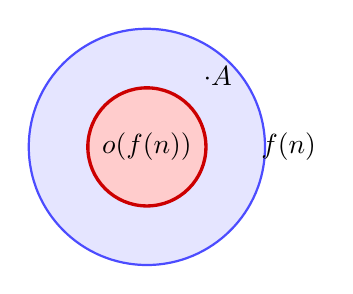
\begin{tikzpicture}
        \draw[
            thick,
            blue!70,
            fill=blue!10
        ] (0, 0) circle (1.5cm);
        
        \node at (1.8, 0) {$f(n)$};
        
        \draw[
            very thick,
            red!80!black,
            fill=red!20
        ] (0, 0) circle (0.75cm);
        
        \node at (0.9, 0.9) {$\cdot A$}; 
        
        \node at (0, 0) {$o(f(n))$}; 
    \end{tikzpicture}
    
    \caption{\textit{SPACE}$(o(f(n))) \subsetneq$ \textit{SPACE}$(f(n))$.}
    \label{fig:subconjunto} 
\end{figure}

Parecido a la situación de un lenguaje libre de contexto, en el caso de los lenguajes regulares, donde se muestra un lenguaje particular que se diferencía por ser libre de contexto pero no regular.\\
Usando la prueba de diagonalización, se construye una máquina de Turing $D$ que decide el lenguaje $A$ con las siguientes propiedades:
\begin{enumerate}
  \item $D$ generará el lenguaje $A$.
  \item $D$ se ejecutará dentro de $f(n)$.
  \item $D$ se diseñará para asegurarse que su lenguaje no pueda implementarse en un espacio menor, para eso se asegura que su lenguaje sea diferente de cualquier lenguaje decidible por una máquina de Turing en un espacio menor.
  \item $D$ se asegurará que no puede ser implementada en $o(f(n))$.
\end{enumerate}

Prueba: Dada una máquina de Turing D donde:
\begin{enumerate}
  \item $D$ corre en espacio $O(f(n))$.
  \item $D$ es cierto que $L(D) \neq L(M)$ para cualquier MT M que corra en espacio $o(f(n))$.
  \item Dejar $A = L(D)$.
\end{enumerate}

El objetivo de esto es mostrar que $A \in SPACE(f(n))$ pero $A \notin SPACE(o(f(n)))$.
\begin{enumerate}
  \item $D$ recibe como entrada $w$
  \item Marcar las celdas de la cinta Problema$f(n)$ donde $n=|w|$; si trata de usar más cinta, rechaza (solo se permitirá que use el espacio $f(n)$ de lo contrario tal vez D no este en $f(n)$). Para asegurarnos de que eso no pase entonces se coloca el $\#$ para delimitar el espacio $f(n)$, si trata de usar más que eso, rechaza.
  \item Si $w \neq <M>$ para alguna máquina de Turing M, rechazar (w no describe nada, solo es un salto). Rechaza a menos que si sea una $w$ que describa una maquina de Turing M.
  %imagen de la cinta 
  \item Simular * $M$ en $w$.\\ Acepta si M rechaza.\\ Rechaza si M acepta.\\ *NOTA: $D$ puede simular $M$ con un factor constante de espacio.
\end{enumerate}
  %imagen de la cinta 
\begin{figure}[h!]
    \centering
    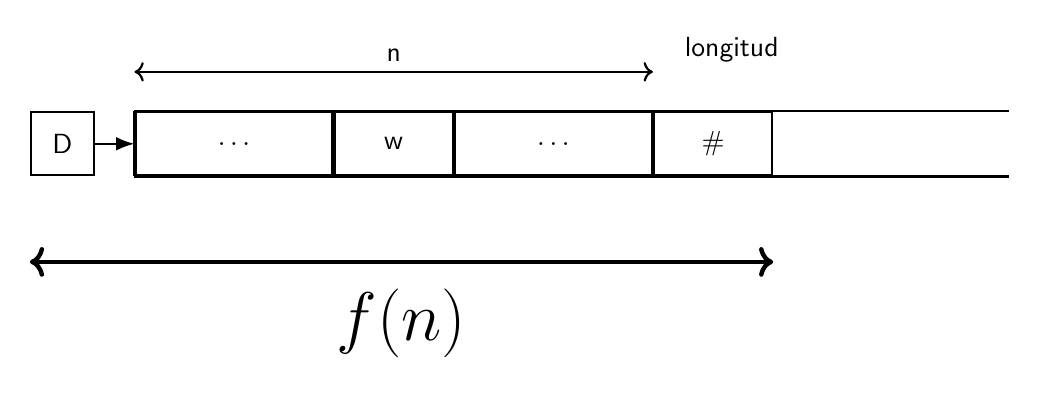
\begin{tikzpicture}[
        every node/.style={font=\sffamily}, % Estilo para todo el texto: sans-serif.
        box/.style={draw=black, thick, rectangle, minimum width=0.8cm, minimum height=0.8cm}, 
        tape/.style={draw=black, thick, rectangle, minimum height=0.8cm}, 
        arrow_style/.style={-Latex, thick, draw=black} 
    ]
        % --- Caja D ---
        \node[box] (D) at (-2,0) {D};

        % --- Celdas de Contenido (Con sus propias cajas y bordes internos) ---
        \node[tape, minimum width=2.5cm, right=0.5cm of D.east, anchor=west] (dots1) {$\dots$};
        \node[tape, minimum width=1.5cm, right=0cm of dots1.east, anchor=west] (w_cell) {w};
        \node[tape, minimum width=2.5cm, right=0cm of w_cell.east, anchor=west] (dots2) {$\dots$};
        \node[tape, minimum width=1.5cm, right=0cm of dots2.east, anchor=west] (hash_cell) {\#};

        % --- Cinta "Abierta" y Larga (Extensión) ---
        
        % 1. Dibujamos la línea de contorno normal, pero solo hasta el borde derecho de la celda #
        %    *NO* usamos 'rectangle', sino líneas individuales.
        \coordinate (tape_north_west) at (dots1.north west);
        \coordinate (tape_south_west) at (dots1.south west);
        \coordinate (tape_north_east_content) at (hash_cell.north east);
        \coordinate (tape_south_east_content) at (hash_cell.south east);

        % 2. Extendemos el borde derecho 3cm más allá de hash_cell.east
        \coordinate (extended_east_north) at ($(hash_cell.north east) + (3cm, 0)$);
        \coordinate (extended_east_south) at ($(hash_cell.south east) + (3cm, 0)$);

        % Dibujamos las líneas:
        % (a) Línea superior: desde el inicio hasta el final extendido
        \draw[thick, draw=black] (tape_north_west) -- (extended_east_north); 
        % (b) Línea inferior: desde el inicio hasta el final extendido
        \draw[thick, draw=black] (tape_south_west) -- (extended_east_south); 
        
        % Esto es crucial: dibuja la línea izquierda que fue omitida por las celdas
        \draw[thick, draw=black] (tape_north_west) -- (tape_south_west);
        
        % ¡OJO!: Las líneas divisorias internas están dadas por el estilo 'tape' de cada nodo.

        % --- Flecha de D a la cinta ---
        \draw[arrow_style] (D.east) -- (dots1.west); 

        % --- Longitud n ---
        \path let \p1 = (dots1.north west), \p2 = (dots2.north east) in
              coordinate (n_start) at (\x1, \y1)
              coordinate (n_end) at (\x2, \y2);
            
        \draw[<->, thick, draw=black] ($(n_start) + (0, 0.5cm)$) 
            -- node[above, font=\sffamily] {n} 
            ($(n_end) + (0, 0.5cm)$)
            node[above, xshift=1cm, font=\sffamily] {longitud}; 

        % --- f(n) (RECTA y TERMINANDO EN #) ---
        
        \coordinate (fn_start_point) at ($(D.west) - (0, 1.5cm)$); 
        % Usamos la coordenada X de hash_cell.east y la Y de fn_start_point para asegurar la rectitud
        \coordinate (fn_end_point) at (hash_cell.east |- fn_start_point); 
            
        \draw[<->, ultra thick, draw=black] (fn_start_point)
            -- node[below=0.2cm, font=\sffamily\bfseries\Huge] {$f(n)$} (fn_end_point); 
            
    \end{tikzpicture}
    \caption{Punto 1. Solo se permitirá que D use el espacio f(n), de lo contrario tal vez D no este en f(n).}
    \label{fig:turing_tape_final_completo}
\end{figure}

$D$ está haciendo algo diferente a $A$, $D$ no puede ser diferente de cada $M$ porque $D$ en sí misma es una máquina de Turing, $D$ solo se ejecuta dentro de celdas $f(n)$ de la cinta, tiene que poder realizar esa simulación de M dentro de esa cantidad de cinta, siempre rechazará si usa más.\\
Si $M$ usa menos que $D$, entonces puede hacer la simulación.
\subsection{Problemas}
\subsubsection{¿Qué pasa si M corre en tiempo o(f(n)) pero tiene una constante grande?}
Entonces $D$ no tendrá espacio para simular $M$ cuando es pequeña.\\
\textit{Solución:} Simular $M$ en infinitos $w's$. Pensando en $w$ como la representación de $M$ pero con un número ilimitado de ceros finales. Se cambia el punto $3.$ por $3. Si w \neq <M>10^*$ por alguna máquina de Turing M, rechaza.\\ Lo primero que se hará con $w$ es eliminar los ceros finales hasta el último 1 y tomar el resto como la descripción de la máquina. Si $M$ de verdad esta corriendo en $o(f(n))$ entoces habrá espacio suficiente para que $M$ se ejecute completamente sobre $w$ y así diferenciarlo de él.\\
%imagen de la cinta
\begin{figure}[h!]
    \centering
    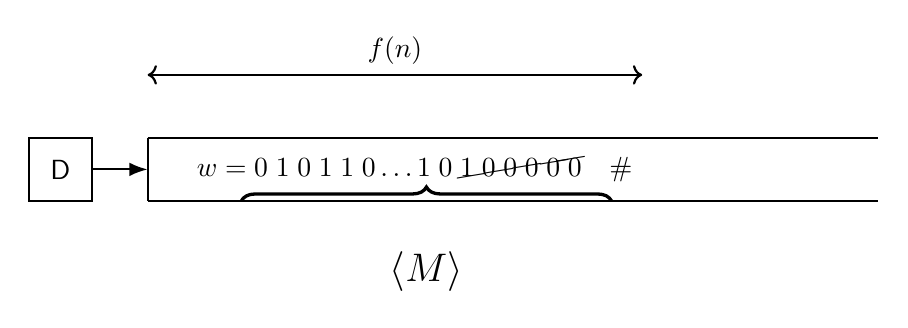
\begin{tikzpicture}[
        every node/.style={font=\sffamily},
        box/.style={draw=black, thick, rectangle, minimum width=0.8cm, minimum height=0.8cm}, 
        arrow_style/.style={-Latex, thick, draw=black} 
    ]
        % --- Caja D ---
        \node[box] (D) at (-2,0) {D};

        % --- Cinta Principal (Contenido y Coordenadas) ---
        \node[font=\sffamily] (content) at (2.5, 0) {$w = 0\; 1\; 0\; 1\; 1\; 0 \dots 1\; 0\; \cancel{1\; 0\; 0\; 0\; 0\; 0}  \quad \#$};
        
        \def\tapeHeight{0.4cm}
        \def\extensionLength{3cm} 

        \coordinate (content_west) at (content.west);
        \coordinate (content_east) at (content.east);

        % Puntos de inicio y fin de la cinta
        \coordinate (tape_start_top) at ($(content_west) + (-0.5cm, \tapeHeight)$);
        \coordinate (tape_start_bottom) at ($(content_west) + (-0.5cm, -\tapeHeight)$);
        
        % Puntos del final extendido de la cinta
        \coordinate (tape_end_top) at ($(content_east) + (\extensionLength, \tapeHeight)$);
        \coordinate (tape_end_bottom) at ($(content_east) + (\extensionLength, -\tapeHeight)$);
        
        % Dibujamos las líneas de la cinta (rectas, sin líneas internas)
        \draw[thick, draw=black] (tape_start_top) -- (tape_start_bottom); % Línea vertical izquierda
        \draw[thick, draw=black] (tape_start_top) -- (tape_end_top);     % Línea superior (recta)
        \draw[thick, draw=black] (tape_start_bottom) -- (tape_end_bottom); % Línea inferior (recta)

        % --- Flecha de D a la cinta ---
        \draw[arrow_style] (D.east) -- (tape_start_top |- D.east); 

        % --- f(n) (RECTA y DESENCIMADA) ---
        \def\fnHeight{0.8cm}
        
        \coordinate (fn_start_point) at ($(tape_start_top) + (0, \fnHeight)$); 
        \coordinate (fn_end_point) at ($(content_east) + (0, \fnHeight + \tapeHeight)$); 
        
        \draw[<->, thick, draw=black] (fn_start_point)
            -- node[above, font=\sffamily] {$f(n)$} (fn_end_point);

        % --- Codificación <M> (ARCO INFERIOR, AJUSTADO AL RANGO 0...0) ---
        
        % COORDENADAS AJUSTADAS para abarcar el código binario
        \coordinate (M_start) at (0.3, 0); % Inicia justo antes del primer '0'
        \coordinate (M_end) at (5.0, 0);   % Termina justo después del último '0'
        
        % Dibuja el corchete curvo (brace) y la etiqueta
        \draw[decorate, decoration={brace, amplitude=5pt, mirror}, very thick] 
            (M_end |- tape_start_bottom) -- (M_start |- tape_start_bottom) 
            node[midway, below=0.5cm, font=\Large] {$\langle M \rangle$};
            
    \end{tikzpicture}
    \caption{Problema 2.2.1 <M> abarca desde el primer 0 hasta el último 0, y se debe de tachar desde el último 0 hasta el último 1.}
    \label{fig:codificacion_m_final_perfecto}
\end{figure}

Ahora $M$ se ejecuta en una gran entrada, suficientemente grande para que $D$ (que tiene más espacios) pueda ejecutarse completamente vacía.
\subsubsection{¿Qué pasa si M se cicla?} D debe detenerse.
Solución: Detener $M$ si corre en $2^{f(n)}$ pasos.\\
*Modificando el paso 4. por 4. Simular * $M$ en $w$ por $2^{f(n)}$ pasos. Acepta si M rechaza. Rechaza si M acepta o no se ha detenido.
\subsubsection{¿Cómo computar f?} $f$ tiene que ser computable dentro del espacio.\\
Solución: Asumir que $f$ es un espacio constructible, i.e. puede computar $f$ con $O(f(n))$. Ciertas funciones como $log_n, log^2_n, n, n^2, 2^n,...$ son espacios constructibles.\\ ¿Se puede decir que $D$ tiene como entrada $M$ y simula $M$ sobre sí mismo? Cierto.

\section{Teorema del Tiempo}
\begin{definition}
Sea $t:\mathbb{N} \rightarrow \mathbb{N}$ una función construible en tiempo. 
Entonces existe un lenguaje $A$ tal que es decidible en tiempo $O(t(n))$ 
pero no es decidible en tiempo $o\!\left(\frac{t(n)}{\log t(n)}\right)$. \cite[p. 341]{sipser2006}

\end{definition}
El teorema de jerarquía temporal establece que, bajo condiciones razonables, 
disponer de más tiempo permite decidir más lenguajes. De manera precisa, 
si $t(n)$ es una función construible en tiempo, entonces existe un lenguaje 
que puede ser decidido en tiempo $O(t(n))$, pero que no puede ser decidido 
en tiempo 
$o\!\left(\dfrac{t(n)}{\log t(n)}\right)$. 

% Este teorema es análogo al teorema de jerarquía espacial, pero incorpora 
% una diferencia fundamental: en el caso del tiempo, simular una máquina de Turing 
% dentro de otra introduce una sobrecarga adicional de tipo logarítmico, 
% lo cual explica la presencia del factor $\log t(n)$ en el denominador.

Para demostrar el teorema, se define una MT $D$ diseñada para “diferenciarse” de todas las máquinas que corren en tiempo más pequeño que $t(n)/\log t(n)$. \cite[p. 341]{sipser2006} La idea es la siguiente:

\begin{figure}[h]
\centering
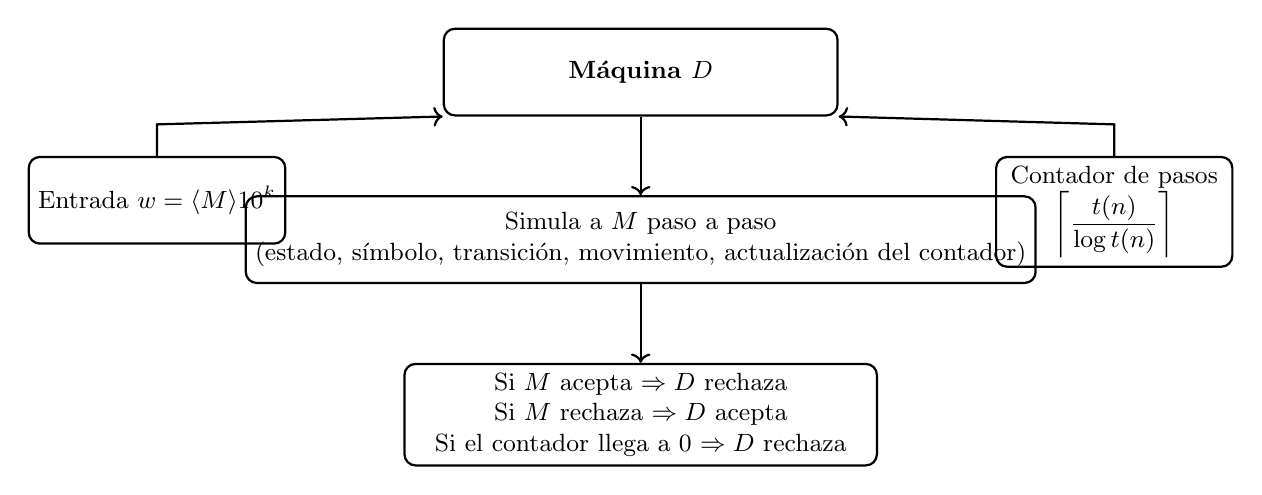
\begin{tikzpicture}[
    box/.style={draw, rounded corners, thick, align=center, minimum height=1.1cm},
    arrow/.style={->, thick},
    font=\small
]

% Caja principal D
\node[box, minimum width=5cm] (D) {\textbf{Máquina $D$}};

% Entrada w
\node[box, below left=0.5cm and 4.5cm of D.south, minimum width=2.0cm] (entrada)
{Entrada $w = \langle M\rangle 10^{k}$};

% Contador
\node[box, below right=0.5cm and 4.5cm of D.south, minimum width=3.0cm] (contador)
{Contador de pasos \\ $\displaystyle \left\lceil \frac{t(n)}{\log t(n)} \right\rceil$};

% Flechas a D
\draw[arrow] (entrada.north) -- ++(0,0.4) -- (D.south west);
\draw[arrow] (contador.north) -- ++(0,0.4) -- (D.south east);

% Caja interna: simulación paso a paso
\node[box, below=1.0cm of D, minimum width=7cm] (simulacion)
{Simula a $M$ paso a paso \\ (estado, símbolo, transición, movimiento, actualización del contador)};

% Flecha hacia simulación
\draw[arrow] (D) -- (simulacion);

% Caja final: decisión
\node[box, below=1.0cm of simulacion, minimum width=6cm] (decision)
{Si $M$ acepta $\Rightarrow D$ rechaza \\ Si $M$ rechaza $\Rightarrow D$ acepta \\ Si el contador llega a 0 $\Rightarrow D$ rechaza};

% Flecha hacia decisión
\draw[arrow] (simulacion) -- (decision);

\end{tikzpicture}

\caption{Esquema de la simulación temporal realizada por la máquina $D$. 
La máquina calcula $t(n)$, establece un contador de pasos 
y simula a $M$ sin exceder el tiempo permitido.}
\end{figure}


\begin{enumerate}
    \item $D$ recibe como entrada una cadena de la forma
    \[
        w = \langle M \rangle 1 0^{k},
    \]
    es decir, codificación de una máquina $M$ seguida de un $1$ y varios ceros. 

    \item $D$ calcula el valor $t(n)$, donde $n = |w|$, utilizando el hecho de que $t(n)$ es construible.

    \item $D$ simula a la máquina $M$ sobre la misma entrada $w$, con límite de tiempo igual a $t(n)$.

    \item Cuando la simulación termina antes de agotar el tiempo, $D$ responde lo opuesto a lo que responde $M$:
    \begin{itemize}
        \item si $M$ acepta, $D$ rechaza;
        \item si $M$ rechaza, $D$ acepta.
    \end{itemize}
\end{enumerate}

Esta técnica es un ejemplo clásico de \textit{diagonalización}.


La diferencia entre el teorema de tiempo y el de espacio aparece cuando analizamos 
el costo de la simulación.

Simular un solo paso de una máquina $M$ requiere que $D$:
\begin{itemize}
    \item Lea el estado actual de $M$, consulte el símbolo bajo la cabeza,busque la transición correcta, escriba el nuevo símbolo, mueva la cabeza, y actualice un contador de pasos disponibles.
\end{itemize}

Este contador debe almacenar un número de tamaño aproximadamente 
$\log t(n)$, y cada actualización requiere tiempo proporcional a ese tamaño. 
Por lo tanto, cada paso simulado aporta un costo adicional de:
\[
O(\log t(n)).
\]

Como consecuencia, para que la simulación complete al menos $g(n)$ pasos de $M$, 
debe cumplirse:
\[
g(n)\cdot \log t(n) \leq t(n).
\]

Esto implica:
\[
g(n) \leq \frac{t(n)}{\log t(n)}.
\]

Esa es la razón exacta por la cual el resultado establece una separación entre:
\[
\text{TIME}(t(n))
\qquad \text{y} \qquad
\text{TIME}\!\left( o\!\left( \frac{t(n)}{\log t(n)} \right) \right).
\]

\begin{corollary}[Corolario 9.11] \cite[p. 343]{sipser2006} \mbox{}\\[-0.8em]
Para cualesquiera dos funciones $t_1, t_2 : \mathbb{N} \rightarrow \mathbb{N}$, donde 
$t_1(n)$ es $o\!\left(\dfrac{t_2(n)}{\log t_2(n)}\right)$ y $t_2$ es construible en tiempo,
\[
\text{TIME}(t_1(n)) \subsetneq \text{TIME}(t_2(n)). 
\]
\end{corollary}
Este corolario formaliza la idea de que si una función de tiempo crece 
suficientemente más rápido que otra, entonces la clase de lenguajes que puede decidir con ese tiempo mayor es 
estrictamente más amplia. Es una consecuencia directa del teorema de jerarquía temporal, 
aplicado a dos funciones específicas.

\begin{corollary}[Corolario 9.13] \cite[p. 343]{sipser2006}
\[
\mathbf{P} \subsetneq \mathbf{EXPTIME}.
\]
\end{corollary}
Este corolario es uno de los resultados más importantes derivados de la jerarquía temporal.
Como la función $2^{n}$ crece mucho más rápido que cualquier polinomio, el teorema implica 
que existe al menos un lenguaje decidible en tiempo exponencial, pero no en tiempo polinomial.

Así se demuestra que la clase de problemas que pueden resolverse en tiempo polinomial 
es estrictamente más pequeña que la clase de problemas que pueden resolverse en tiempo 
exponencial. En otras palabras, existen problemas que son decidibles pero intratables, 
pues requieren un tiempo exponencial para ser resueltos.
\subsection{Preguntas clave}
\subsubsection{¿Por qué necesitamos que t(n) sea “construible en tiempo”}\mbox{}\\[-0.1em]
\textit{Solución:} Porque D necesita calcular t(n) para saber cuánto tiempo puede usar.
Si t(n) no pudiera calcularse dentro de t(n) tiempo, la máquina D no podría limitarse correctamente y toda la prueba se caería.

\subsubsection{¿Qué pasa si la máquina M corre en tiempo o(t(n)) pero con una constante tan grande que D no alcanza a simularla completamente?}\mbox{}\\[-0.8em]

Si M efectivamente es “más rápida”, pero sus tiempos para entradas pequeñas son enormes, podría parecer que D no puede simularla dentro del límite t(n).

\textit{Solución:}  
Usamos entradas del tipo $\langle M \rangle 1 0^{*}$ para alargar artificialmente la entrada.  
Al aumentar la longitud $n$, la cota $t(n)$ también crece, y eventualmente será suficiente 
para simular por completo a $M$ en esa entrada alargada.  
Por eso la diagonalización no falla: siempre existe una entrada lo bastante grande para 
distinguir $A$ del lenguaje de $M$.

\section{Clases de Complejidad Exponencial y la Completitud de $EQ_{REX\uparrow}$}
Véase la sección de Preliminares, donde se introducen las nociones de $EXPSPACE-completitud$ y $EXPTIME-completitud$. De manera semejante a la 
definición de $EXPSPACE-completitud$ (Definición~\ref{def:expspace-completo}:), la noción correspondiente para $EXPTIME-completitud$ (Definición~\ref{def:exptime-completo}) es completamente análoga.

Los teoremas jerarquia demuestran que
$$PSPACE \subsetneq EXSPACE$$
$$P \subsetneq EXPTIME$$
Partiendo de esta separación estricta, podemos deducir la intractabilidad de los problemas completos. Si un problema $EXPSPACE-completo$ pudiera resolverse en tiempo polinómico ($P$), entonces, debido a la propiedad de las reducciones polinómicas, todos los problemas de $EXPSPACE$ podrían resolverse en tiempo polinómico.

Esto implicaría que $EXPSPACE\subseteq P$, causando que la jerarquía colapse y contradiciendo el teorema que establece que EXPSPACE es estrictamente mayor que $P$. Por lo tanto, es imposible que existan algoritmos eficientes para estos problemas; son demostrablemente intratables.

A continuación se mostrará un problema $EXPSPACE-completo$.

\begin{theorem}
	Sea $EQ_{REX\uparrow} = \{ \langle R_1, R_2 \rangle \mid R_1 \text{ y } R_2 \text{ son expresiones regulares con exponenciación y } L(R_1) = L(R_2) \}$. $EQ_{REX\uparrow}$ es $EXPSPACE-completo$\cite[p. 4]{cita3}\cite[p. 344]{sipser2006}
\end{theorem}
\begin{proof}
	\begin{enumerate}
		\item $EQ_{REX\uparrow} \in EXPSPACE$
		\item Si $A \in EXPTIME$ entonces $A \leq_p EQ_{REX\uparrow}$ 
	\end{enumerate}

	\textbf{$EQ_{REX\uparrow} \in EXPSPACE$}\\
	Sea $n$ la longitud de la entrada $\langle Q, R \rangle$.
	\begin{enumerate}
		\item Expandimos todas las exponenciaciones en $Q$ y $R$ para obtener expresiones regulares estándar $Q'$ y $R'$.
		\item Dado que los exponentes están en binario, el valor máximo de un exponente es $2^n$. La longitud de las expresiones expandidas es a lo sumo $O(n \cdot 2^n)$.
		\item Convertimos $Q'$ y $R'$ a Autómatas Finitos No Deterministas (NFA) $N_Q$ y $N_R$. El número de estados de cada autómata es lineal respecto a la longitud de la expresión, es decir, $O(n \cdot 2^n)$.
		\item Verificamos si $L(N_Q) = L(N_R)$. Sabemos que la equivalencia de NFAs se puede decidir en espacio polinómico respecto al tamaño de los autómatas (usando el algoritmo de no-equivalencia y el Teorema de Savitch.
		\item El espacio requerido es $O((\text{tamaño})^2) = O((n \cdot 2^n)^2) = O(2^{2n+2 \log n})$, lo cual pertenece a la clase $EXPSPACE$.
	\end{enumerate}

	\textbf{Si $A \in EXPTIME$ entonces $A \leq_p EQ_{REX\uparrow}$}\\
	Sea $A$ un lenguaje arbitrario en EXPSPACE decidido por una Máquina de Turing determinista $M$ que utiliza espacio $2^{n^k}$ para alguna constante $k$. Dada una entrada $w$, construimos en tiempo polinómico dos expresiones regulares $R_1$ y $R_2$ tales que:

	Construcción:
	\begin{itemize}
		\item $R_1 = \Sigma^*$ (Genera todas las cadenas).
		\item $R_2$ generará todas las cadenas que no son historias de computación de rechazo válidas de $M$ sobre $w$.
	\end{itemize}
	Si $M$ acepta $w$, no existe historia de rechazo, por lo que $L(R_2) = \Sigma^* = L(R_1)$. Si $M$ rechaza, existe una historia válida $h$, y $L(R_2) = \Sigma^* \setminus \{h\} \neq L(R_1)$.
	\\

	\textbf{Construcción Detallada de $R_2$}
	Una cadena falla en ser un historial de rechazo si viola al menos una de las condiciones de validez: inicio, transición o finalización.

	\paragraph{1. Mal Inicio ($R_{\text{bad-start}}$)}
	Debe generar cualquier cadena que no comience con la configuración inicial $C_1 = q_0 w_1 \dots w_n \sqcup \dots \sqcup \#$. Sipser descompone esto en la unión de varios errores posibles:
    \

	Donde $\Delta$ es el alfabeto y $\Delta_{-x}$ denota $(\Delta \setminus \{x\})$.
	\begin{itemize}
		\item $S_0 = \Delta_{-q_0} \Sigma^*$: El primer símbolo no es el estado inicial $q_0$.
		\item $S_i = \Sigma^i \Delta_{-w_i} \Sigma^*$: El símbolo en la posición $i+1$ no coincide con la entrada $w_i$ (para $1 \le i \le n$).
		\item $S_b$: Detecta si los símbolos de relleno (blancos) no son correctos. Aquí la exponenciación es conveniente para saltar hasta la zona de blancos, pero en $S_{\#}$ se vuelve crucial.
		\item $S_{\#} = \Sigma^{\uparrow 2^{n^k}} \Delta_{-\#} \Sigma^*$: El símbolo en la posición $2^{n^k}+1$ (donde termina la primera configuración) no es el separador $\#$. Usamos $\Sigma^{\uparrow 2^{n^k}}$ para avanzar exactamente la longitud de una configuración.
    \end{itemize}

	\paragraph{2. Mal Movimiento ($R_{\text{bad-window}}$)}
	Esta subexpresión detecta si la configuración $C_{t+1}$ no se sigue válidamente de $C_t$. En una MT, el contenido de una celda en $t+1$ está determinado localmente por una ventana de 3 celdas en $t$ (izquierda, actual, derecha).
    
	Si en $C_t$ tenemos la secuencia de símbolos $abc$, y la función de transición de $M$ dicta que el símbolo central debe convertirse en $d$, entonces hay un error si en $C_{t+1}$ encontramos un símbolo $d' \neq d$ en la posición correspondiente.
    
    	La dificultad radica en que, en la cadena lineal del historial, la posición correspondiente en $C_{t+1}$ está separada por exactamente $2^{n^k}$ símbolos.
	\
	Sin el operador $\uparrow$, tendríamos que escribir $2^{n^k}-1$ símbolos comodín para conectar $abc$ con el error $d'$. Esto haría que la expresión regular tuviera longitud exponencial, invalidando la reducción polinómica. Al usar un exponente binario, representamos el número $2^{n^k}$ con $O(n^k)$ bits, manteniendo el tamaño de $R_2$ polinómico respecto a $n$.

    	\paragraph{3. Mal Final ($R_{\text{bad-reject}}$)}
	Genera cadenas que no contienen el estado de rechazo $q_{reject}$:
	\

	Como $R_1$ y $R_2$ se construyen en tiempo polinómico y capturan la aceptación de $M$, $EQ_{REX\uparrow}$ es $EXPSPACE-completo$.
\end{proof}i
\section{Conclusiones}
En este trabajo se ha visto cómo los recursos computacionales, tiempo y espacio, son valiosos. Ofrecer más recursos incrementa el conjunto de problemas que pueden ser resueltos. Los Teoremas de Jerarquía del Espacio y del Tiempo formalizan esta intuición, utilizando la técnica de diagonalización para construir un lenguaje que deliberadamente evita ser resuelto por una máquina con menos recursos.

El Teorema de Jerarquía del Espacio prueba que basta con un poco más de espacio disponible (siempre que sea una cantidad que la máquina pueda medir, conocida como "espacio constructible") para decidir un conjunto estrictamente mayor de lenguajes. En otras palabras, la clase de problemas que se pueden resolver con la función $f_1(n)$ es un subconjunto estricto de la clase que se resuelve con la función $f_2(n)$ si $f_2$ crece más rápido.

El Teorema de Jerarquía del Tiempo establece una separación análoga. Sin embargo, su demostración es más exigente. Para asegurar que la máquina con más tiempo puede "superar" a la máquina más rápida, la ventaja de tiempo debe ser significativamente mayor, debido al factor logarítmico que surge del costo de simular máquinas paso a paso.

Ambos resultados demuestran de manera irrefutable que las clases de complejidad no colapsan y que la potencia computacional aumenta de manera estricta conforme se incrementan los recursos disponibles.

La consecuencia más significativa de esta jerarquía es la demostración de la intratabilidad. Al probar que $P$ es estrictamente menor que $EXPTIME$, los teoremas nos dicen que existen problemas cuya solución requiere, inherentemente, cantidades enormes de tiempo o espacio (exponencial), haciéndolos impracticables incluso aunque sean teóricamente decidibles. La estructura jerárquica de la complejidad es, por tanto, el fundamento que distingue a los problemas eficientemente resolubles de aquellos que están, demostrablemente, fuera del alcance de la computación práctica.


% ----------- 5. BIBLIOGRAFÍA -----------
\bibliographystyle{ACM-Reference-Format}
\bibliography{referencias} % Llama al archivo referencias.bib

\end{document}
